\documentclass[a4paper,11pt]{article}
\usepackage[T1]{fontenc}
\usepackage[utf8]{inputenc}
\usepackage{lmodern}
\usepackage{graphicx}
\usepackage{url}
\newcommand{\tabcaption}{\def\@captype{table}\caption}
\title{
Mining of Massive Dataset\\
Project 2 Report
}
\author{Hao Jiteng, Zhou Lizhi, Yang Fangzhou}

\begin{document}

\maketitle
%\tableofcontents

\begin{abstract}
K-means is a simple yet useful clustering algorithm. It's underlying natural
implies that it could be parallelized or distributized. Some implementation of
kmeans employs platforms such as Hadoop and CUDA to boost the process of mining
of massive dataset.

In our project we implement k-means algorithm on Apache Hadoop Project. We ran
our algorithm on our tiny cluster. Evaluation has been done to measure our
algorithm.

Our source code and other relative materials could be found in github~\cite{github:source}
\end{abstract}

\section{Introduction}
\subsection{Hadoop}
Following is the introduction of Hadoop on its project
homepage~\cite{apache:hadoop}.

The Apache™ Hadoop™ project develops open-source software for reliable,
scalable, distributed computing.

The Apache Hadoop software library is a framework that allows for the
distributed processing of large data sets across clusters of computers using a
simple programming model. It is designed to scale up from single servers to
thousands of machines, each offering local computation and storage. Rather than
rely on hardware to deliver high-avaiability, the library itself is designed to
detect and handle failures at the application layer, so delivering a
highly-available service on top of a cluster of computers, each of which may
be prone to failures.

We mainly use the Hadoop MapReduce framework.

\subsection{k-means}
There are many materials that introduce k-means
algorithms. MacQueen, J. et al. proposed k-means algorithm in
\cite{algo:kmeans1}. In \cite{algo:kmeans2} the author introduced a simple
k-means MapReduce algorithm. 

The dataset is relatively large comparing to the memory size. Thus we need a
mechanism to deal with the incompatibility of memory. MapReduce is a solution to
this problem. The detail of our algorithm is documented in the following
section.

\section{Clustering Algorithm}
In this section we discuss the k-means clustering algorithm used in our
implementation. Note that to find proper initial clusters, which may lead to
fewer iterations and good result, we also implemented a Canopy clustering
MapReduce algorithm.
\subsection{Canopy Clustering}
Canopy method is a relative easy but efficient clustering method. The basic 
idea of Canopy is to put the similar items into the subset, which are called 
Canopies. Different Canopies can overlap each other, but there is no node, 
which doesn't belongs to any of Canopy. Thus, here we use this method to 
preprocess the dataset and speed up Kmeans method. 

The algorithm is built up by the following MapReduce phases.
\subsubsection{Procedure}
\begin{enumerate}
  \item Mapper \\
      \verb|<LongWritable, Text>|$\rightarrow$ \verb|<1,CanopyCluster>|\\
      Choose two distance threshold $t1$ and $t2$, where $t1>t2$. For each  
      node P in the list, calculate the distance between node 
      P and Canopy, if this distance is less than t1, put P into this 
      Canopy cluster, if no such kind Canopy cluster exits, take P as a new 
      Canopy. If P was near enough to some Canopy cluster, which means the 
      distance   between P and the Canopy is less than t2, delete 
      node P from the list. 
  \item Reducer\\
    \verb|<1,CanopyCluster>|  $\rightarrow$   
    \verb|<identifier,KmeansCluster>| \\
     There is only one reducer and the reducer's job is to do another canopy 
     custering on the output of the mappers described above. That's why the 
     mappers always assign 1 to the keys of every output pair.
     For this round of clustering we can use another $t1,t2$ combination, 
     namely $t3$ and $t4$. 
     It's handy to use the KmeansCluster as the result format and kmeans 
     clustering pass could load the result quickly.
\end{enumerate}


\subsection{k-means Clustering}
Mahout Project~\cite{apache:mahout} is a data mining framework under Apache™
Fundation. It contains a k-means implementation. The blog~\cite{algo:kmeans3}
gives a very detailed view of the algorithm. Our algorithm mainly based on the
idea of Mahout Project. Actually, this algorithm is very similar to the BFR
algorithm in our lectures.

The algorithm is built up by the following MapReduce phases,
\begin{enumerate}
  \item The k-means iteration, output every cluster centroid if
  converged.  	
  \item Assign every point to a known cluster and output the result.
\end{enumerate}

The detail of the first phase is described as follows
\subsubsection{Iterate clusters}
\begin{enumerate}
  \item Mapper\\\verb|<LongWritable, KmeansCluster>|$\rightarrow$
  \verb|<LongWritable,KmeansCluster>|. It reads the input file content as value.
  The key is the value offset in the file. Then it convert the value to a
  VectorDoubleWritable, which is used to represent the feature vector. It finds
  the nearest cluster to the vector, and output cluster id as key, a new cluster
  containing only point as value.
  \item Combiner\\\verb|<LongWritable, KmeansCluster>|$\rightarrow$
  \verb|<LongWritable, KmeansCluster>|. It reads the output from Mapper and
  combine those tuples who have the same cluster id(meaning that they are
  assigned to the same cluster) using KmeansCluster.omitCluster(). This function
  reduced the network transmission flow because the actual meaningful
  information need to be communicated between different nodes are only the N,
  SUM and SUMSQ of clusters, which is described in the lecture slides of BFR 
  algorithm. 
  \item Reducer\\\verb|<LongWritable, KmeansCluster>|$\rightarrow$
  \verb|<LongWritable, KmeansCluster>|. It reads the cluster id as key and the
  KmeansCluster as value. It adds the N, SUM and SUMSQ. The result leads to the
  combination of clusters. Finally the reducer outputs the result clusters of
  this single iteration. This clusters are input of next iteration. During
  reducer, if the movement of one cluster if less than a threshold, it's said
  to be ``Converged''. If a cluster is converged, a counter in context will
  increase by one.
  \item If, in the driver, the counter equals the number of clusters, meaning
  that all clusters are converged, this phase is finished.
\end{enumerate} 
\subsubsection{Assign Point to Clusters}
After the iterations, the clusters are stable. Next we are going to assign every
point to its nearest cluster. This phase only require mapper to do all the
works, since this procedure is highly parallelized. Each two point are
independent of each other.

The mapper takes the following form:\\
\verb|<LongWritable, Text>|$\rightarrow$\verb|<Text, Text>|\\
It takes the data offset in file as key and the data as value. First it convert
the Text object into a VectorDoubleWritble object that represents a data point.
For each point we find the nearest cluster and output the cluster id and some
other useful information for statistic and evaluation as value.

\section{Evaluation}
To evaluate the results of our experiment, we calculate the precision and 
recall of the results, then calculate the F value. Better results we get will 
lead to a better score.

\subsection{Dataset}
\subsubsection{MSRA image data set}
The MSRA image data set contains 295 classes of images. Every image class
has hundreds of images. 7 features are used to describe the images. There are
files that decribe the relavence between the image and the topic.

For our situation, we combine the 7 features into one and regards it as a vector
with about a thousand dimensions. We did't use the relavence information for
simplicity. The evaluation results are shown in Section.~\ref{sec:evaluation}

To deal with the incapability of small memory and slow speed compare to the
dataset, we just pick a subset of the dataset. However, these files contain all
features The files we picked are listed below,\\
\textsf{apple banana blood bus calendar coin console eye face fire gun rock sun
television ufo}

Also, we use a set of different convergence threshold to evaluate the results
and the running time.

\subsection{Cluster Information}
To run our Hadoop, we established a tiny cluster with 3 computer connected by 
a 100Mbps TP-Link router using Ethernet.
\begin{enumerate}
  \item Namenode/DataNode/JobTracker
  \begin{itemize}
    \item Intel Core 2 Duo P8700 @ 2.53GHz
    \item 2 Core 2 Threads
    \item 4G DDR3 1066 RAM
    \item OpenSUSE 12.1 x64
  \end{itemize}
  \item DataNode
  \begin{itemize}
    \item Intel Core 2 Duo T6600 @ 2.2GHz
    \item 2 Core 2 Threads
    \item 2G DDR2 800 RAM
    \item Archlinux i386
  \end{itemize}
  \item DataNode
  \begin{itemize}
    \item AMD Processor @ 3.0GHz 
    \item 6 Core 6 Threads
    \item 8G DDR3 1066 RAM
    \item Ubuntu 12.04 LTS x64
  \end{itemize}
\end{enumerate}
\subsection{Evaluation Results}
\subsubsection{MSRA image dataset}
Results are listed in the table.\ref{tab:evaluation}

\begin{table}[!h]
    \begin{tabular}{l|lll|ll}
        \hline 
        THRESHOLD & PRECISION & RECALL & F & ITERATION & TIME(s)\\
        \hline
        0.01 & 0.08366 & 0.27716 & 0.12853 & 11 & 599.839\\
        0.001 & 0.08335 & 0.26792 & 0.12715 & 20 &  1028.0 \\
        0.0001 & 0.08333 & 0.26202 &  0.12644 & 33 & 1670.715\\
        0.00001 & 0.08334 & 0.26187 &  0.12644 & 38 & 1905.114\\
        0.000001 & 0.08334 & 0.26187 &  0.12644 & 41 & 1960.52\\
        \hline
    \end{tabular}
    \caption{Evaluation Results}
    \label{tab:evaluation}
\end{table}

\begin{figure}[!h]
    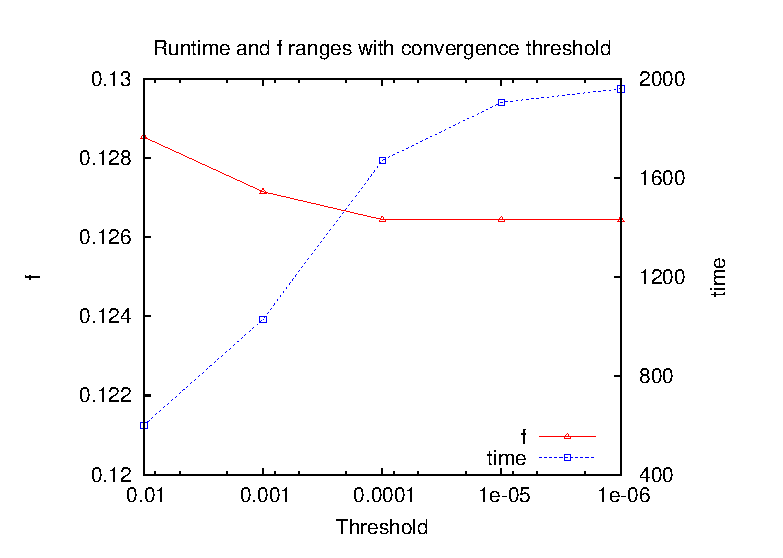
\includegraphics{plot.eps}
    \caption{Evaluation Results}
    \label{fig:evaluation}
\end{figure}

\subsection{Note on the Results}
The results of given dataset are really poor, but we guess the dataset can 
be a problem because the features are actually not relarant to the labels.

We have run some testings on some different datasets whose points can be 
distinguish clearly. Our program gave almost perfect results.

\subsubsection{A-set dataset}
The A-set dataset~\cite{dataset:aset} is used to test our algorithm's
correctness. This dataset is downloaded from the Internet. The visualization of
this data set shows that the data points are relatively seperated, which is very
suitable to verify the correctness of our k-means.

\subsubsection{A-set result}
As we can see in the dataset download webpage~\cite{dataset:aset}, our second
evaluation dataset is quite seperated. It doesn't matter whether using canopy
clustering. The kmeans clustering converge at once with a totally correct
clustering result. It proved that our algorithm and MapReduce clusters are
correct, no matter how bad the result of MSRA image dataset is.

\section{Conclusion}
We finished this project on a own built tiny cluster infrastructure with our own
PC and laptops. We implemented a k-means algorihtm using hadoop framework with
MapReduce. We tested our algorithm on our infrastructure with MSRA image dataset
and 1024 dimension A-set dataset from~\cite{dataset:aset}. The evaluation result
shows that our algirthm is correct and converges fast although there are some
inaccuraccies when using the MSRA data set.

\bibliographystyle{plain}
\bibliography{myrefs.bib}

\end{document}
